\subsection{背景}

\subsubsection{ゲームを超えたXRへの期待の高まり}

昨今 VR(Virtual Reality)や AR(Augmented Reality)などのXRが世間から注目を浴びている.
IDCの2022年3月のレポート\cite{idc} によると,世界の AR/VR ヘッドセットの市場は2021年で
92.1\% 成長し,1000万台を超えるヘッドセットが出荷された.
また,ヘッドセットの市場は2026年まで年平均35.1\%で成長し,
2026年に出荷されるヘッドセットは5000万台を超えると予想されている(図\ref{fig:idc}).

\begin{figure}[htbp]
  \begin{minipage}[b]{0.50\linewidth}
    \centering
    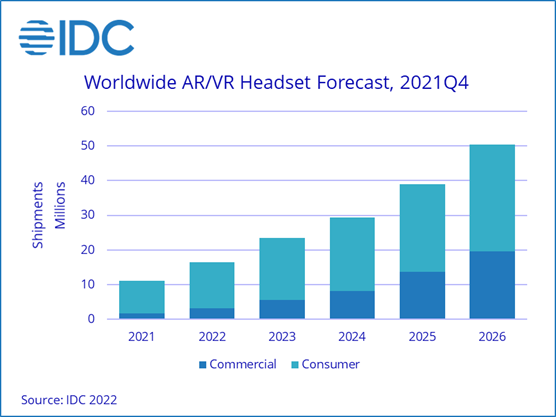
\includegraphics[keepaspectratio, width=0.9\linewidth]{fig/idc.png}
    \caption{IDCによる世界のAR/VRヘッドセットの市場予測}
    \label{fig:idc}
  \end{minipage}
  \begin{minipage}[b]{0.50\linewidth}
    \centering
    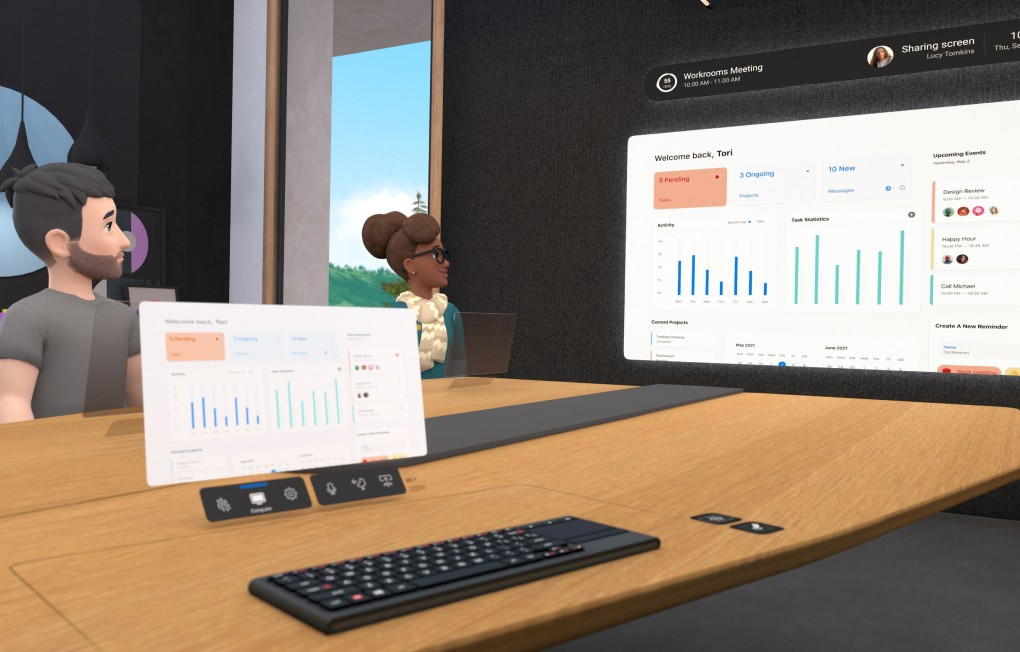
\includegraphics[keepaspectratio, width=0.9\linewidth]{fig/workrooms.jpeg}
    \caption{Horizon Workrooms (Meta社)}
    \label{fig:workrooms}
  \end{minipage}
\end{figure}

特に2021年はメタバースへの期待が高まった年であり,同年10月の Facebook 社の社名変更などから
もうかがえ,XRは従来のゲーム利用を超えた,より幅広い日常生活での利用が期待されている.
Meta社は特に
"Infinite Office\footnote{Infinite Office - Meta Quest:\url{https://www.youtube.com/watch?v=5_bVkbG1ZCo&t=1s}}"
のコンセプトのもと,ビジネス会議用VRアプリ,Horizon Workroom
\footnote{Horizon Workrooms - Meta Quest:\url{https://www.oculus.com/workrooms/}}
(図\ref{fig:workrooms})を発表し,仕事・作業のためのXR空間の重要性が示唆されている.

% コロナ・リモートワークの影響を書いてもいい

\subsubsection{通常の2Dデスクトップ環境におけるWindowing Systemについて}

今日において GUI デスクトップ環境ではWindowing System
(Linuxでは X11やWayland,macOSではQuartz compositorなど)が用いられており,
これによって優れた作業環境を提供できている.
Windowing Systemではアプリケーションが直接自身の描画内容をディスプレイに出力したり,
マウスなどのインプットデバイスからの入力を受け取ったりせず,ディスプレイサーバや
コンポジッタと呼ばれるソフトウェアとのやりとり(プロセス間通信)を介して
これらのハードウェアを扱うようにしている(図\ref{fig:2d-windowing-system}).
コンポジッタの主な役割は,
\begin{itemize}
  \item 複数のアプリケーションから描画内容を受け取り,
        それらを一枚のスクリーンに合成してディスプレイに表示する.
  \item マウスやキーボードなどのハードウェアからの入力を適切なアプリケーション
        (ユーザがフォーカスしているアプリケーションなど)に割り振る.
  \item ドラッグ\&ドロップなどのアプリケーション間のデータ共有の仕組みを提供する.
\end{itemize}
などである.これによって,開発元の異なる複数のアプリケーションを同じディスプレイ上にウィンドウが
自然に重なる形で表示したり,また1つのマウスやキーボードでフォーカスを切り替えながら複数の
アプリケーションを操作したりでき,マルチアプリケーション・マルチタスクの環境が実現されている.

\begin{figure}[htbp]
  \begin{minipage}[t]{0.50\linewidth}
    \centering
    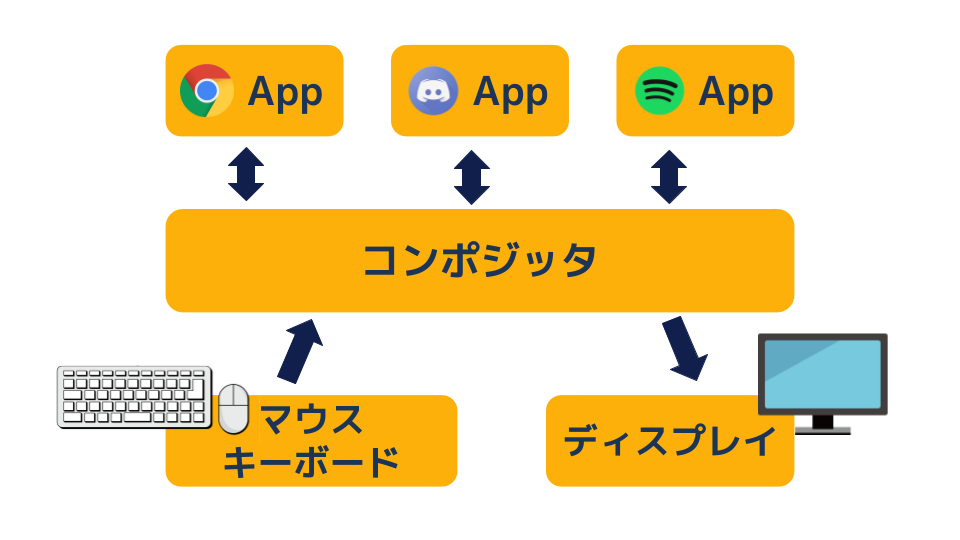
\includegraphics[keepaspectratio, width=\linewidth]{fig/2d-windowing-system.png}
    \caption{2D Windowing Systemの概要図}
    \label{fig:2d-windowing-system}
  \end{minipage}
  \begin{minipage}[t]{0.50\linewidth}
    \centering
    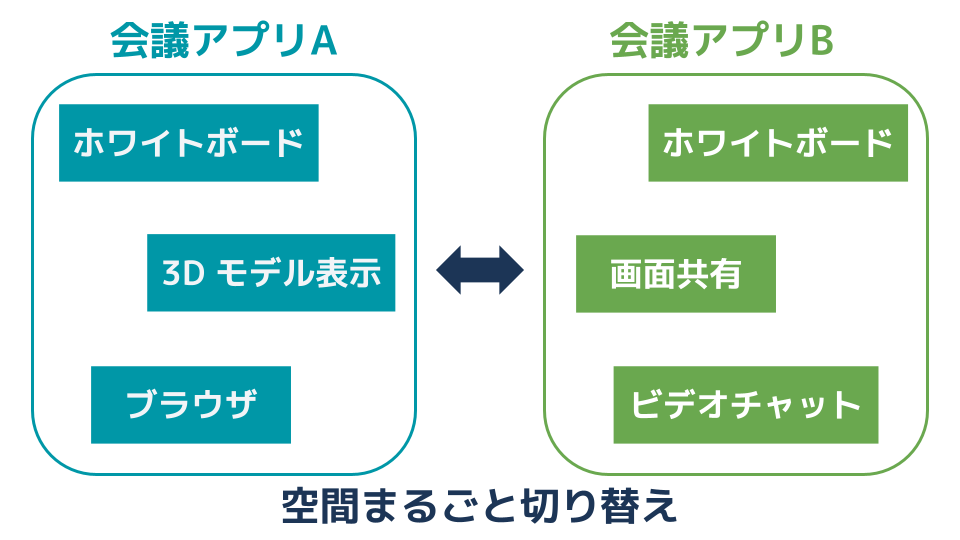
\includegraphics[keepaspectratio, width=0.9\linewidth]{fig/xr-app-switch.png}
    \caption{
      現状のXRアプリケーションの切り替え.アプリケーションの切り替えは,空間内の全ての
      機能を切り替えることになってしまう.
    }
    \label{fig:xr-app-switch}
  \end{minipage}
\end{figure}

\subsubsection{現状のXRアプリケーションについて}

2Dのデスクトップ環境では複数のアプリケーションが同時に使用・連携できるのに対し,
現状のXRアプリケーションは基本的に1つのメインアプリケーションがユーザの視界の全てを支配する.
そのため,アプリケーションを切り替えると,空間ごと切り替えることに
なってしまい(図 \ref{fig:xr-app-switch}),XRアプリケーションは,その空間に必要な
機能をその1つのアプリケーションが全て実装している必要がある.
1つのアプリケーションが1つの世界観を作り出すXRゲームなどにおいてはこれで問題ないが,
作業空間としてXRを用いたい場合は問題が生じる.
作業空間に必要な機能は個人ごとに大きく異なり多様性が大きいため,1つのアプリケーションが
全てのニーズに応えて機能を実装するのは現実的に不可能である.
例えば図\ref{fig:xr-app-switch}の例で,会議アプリAを利用しているユーザが会議アプリBの
画面共有のような機能を3Dモデルの表示と一緒に使いたいと思っても,
会議アプリAの開発元が画面共有機能を追加しない限りそれは不可能である.

一部のXR空間では簡易的に複数のアプリケーションを重ねて表示する機能を提供する仕組みも存在するが,
それについては\ref{section:openxr-overlay}で詳しく言及する.
% また特に,このような汎用的な会議アプリケーションに対して,ニーズの割合が小さい,例えば
% 医療CTスキャンの結果を表示するようなアプリケーションは実装されないだろう.
% そして逆に医療CTスキャンの結果を表示したいモチベーションの開発者が同時に会議アプリケーション
% としての機能を実装することもないと考えられるため,XR会議をしながらCTスキャンの結果を
% 見るという世界が実現する可能性は低い.

\subsubsection{何が必要か}

特に作業空間としてのXRでは,全ての機能を1つのアプリケーションが実装するのではなく,
図\ref{fig:xr-app-install}のように個々の機能がそれぞれアプリケーションとして
異なる開発元によって開発され,ユーザが必要な機能のアプリケーションをインストールすることで
自分に最適な作業空間を作れるようにするべきである.
% textlint-disable
このようにお気に入りのアプリケーションをインストールし,複数のアプリケーションを同時に
% textlint-enable
利用することで作業空間を作り上げていくことは,2Dのデスクトップ環境では当然のように
行われていることだが,XRの作業空間では達成できていない.
XRにもこのようなマルチアプリケーション・マルチタスクの作業環境が求められる.

\begin{figure}[htbp]
  \begin{minipage}[t]{0.50\linewidth}
    \centering
    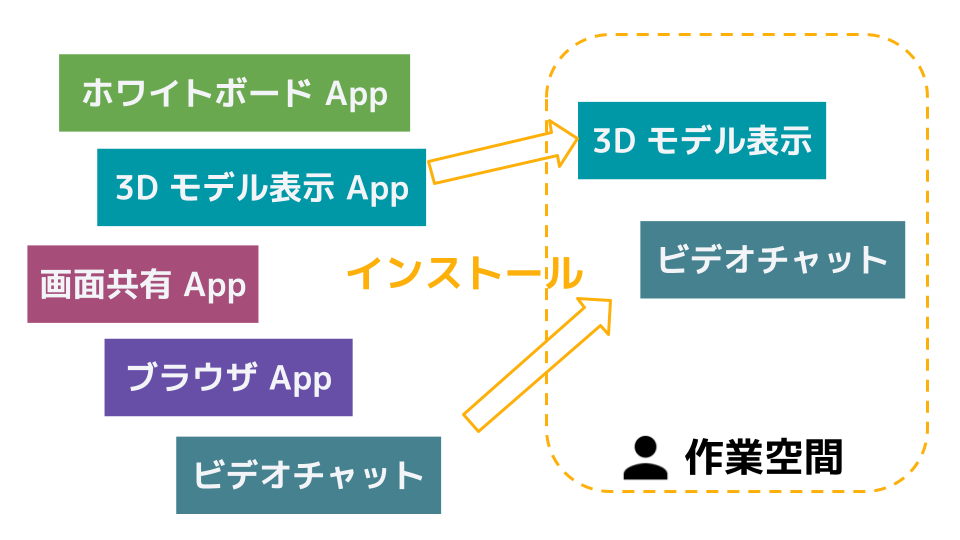
\includegraphics[keepaspectratio, width=\linewidth]{fig/xr-app-install.png}
    \caption{XR空間でユーザが好きなアプリケーションをインストールして同時に複数使う.}
    \label{fig:xr-app-install}
  \end{minipage}
\end{figure}
